\documentclass{jsarticle}
\usepackage[dvipdfmx]{graphicx,color}
\usepackage{amsmath}
\begin{document}

\title{ALIS whitepaper}
\author{Masahiro Yasu and Sota Ishii and Takashi Mizusawa}
\maketitle

\section{目次}
\begin{itemize}
	\item ALISとは
	\item 我々が狙うマーケット規模と日本マーケットの魅力
	\item 日本におけるプラットフォームのグロース戦略
	\item プラットフォームの紹介と特徴
	\item なぜ良質な記事が集まるのか
	\item なぜ人々に価値を還元できるのか
	\item なぜALISは長期的な発展を続けることができるのか
	\item トークンはどのように作成・配布するのか
	\item 詳細の配布ロジックとパラメータの調整について
	\item 不正はどうやって防ぐのか
	\item ALISで用いるブロックチェーン技術について
	\item チームのビジョン・ミッションおよびチームメンバーの詳細プロフィール
	\item ファイナンス
	\item お金の使い道
	\item 企業の運営方針
	\item なぜ香港でICOを実施するのか
	\item 結論
\end{itemize}
\section{ALISとは}
\begin{center}
	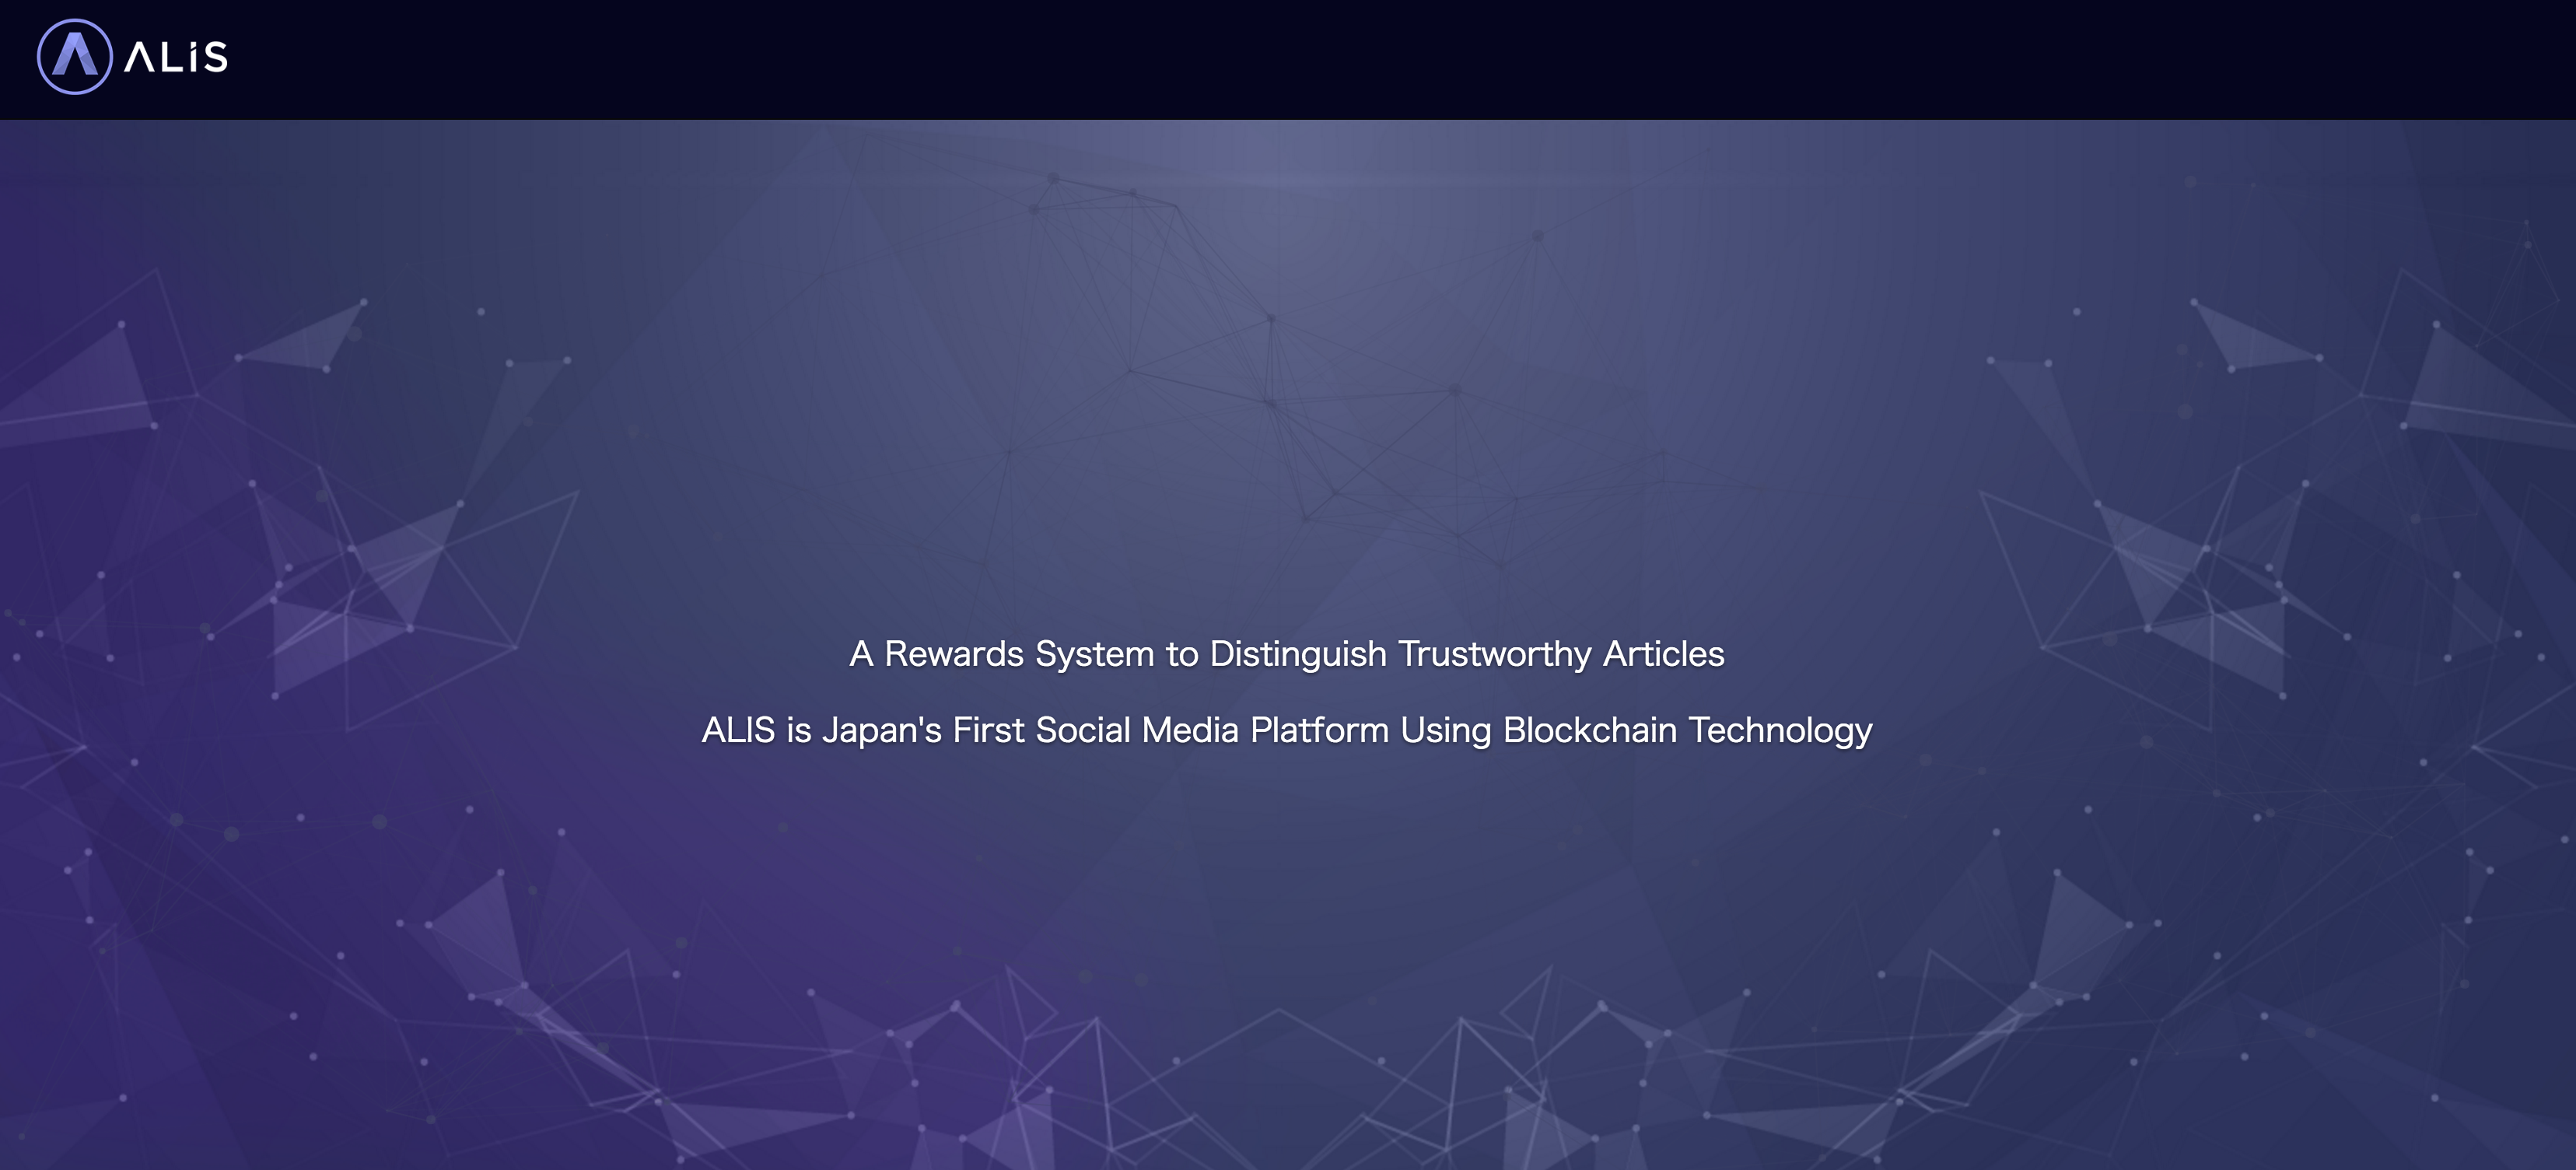
\includegraphics[scale=0.25]{img/aliscover.png}
\end{center}
ALISとは、日本初の分散型ソーシャルメディアプラットフォームである。人々が価値があると思う記事を
多くの個人が生み出す・発見することを可能にする全く新しいソーシャルメディアである。ALISトークンという報酬をキードライバーとして、
従来の広告やステルスマーケティングまがいの記事を排除し、質の高い記事や信頼できる個人に素早くリーチできることを実現する。
正直に言うと、我々はSTEEM(https://steem.io)に
大きな感銘を受けたところからこのプラットフォームの構想をスタートした。STEEMに関する説明に関しては、こちらの記事
(https://cointelegraph.com/news/steemit-new-social-media-platform-which-pays-you-to-post)がわかりやすいためぜひ参照してほしい。
我々のストーリーは、プロジェクトメンバーであるSota Ishiiが数枚の旅行の写真を 
STEEMに掲載(https://steemit.com/japanese/@sot528/1-south-america-tour-no-1)したことから始まる。
なんとその記事はわずか一日で\$30近くの評価を得ることができ、我々は無事そのお金を使って
ドミノピザの最高級ピザを堪能することができた。

\begin{center}
	\includegraphics[scale=0.15]{img/pizza.png} \\
	STEEMの報酬で購入したドミノ・ピザ
\end{center}

我々は強烈な衝撃を受けるとともになぜこのような仕組みが
実現出来ているのかを知りたくなり、徹底的にSTEEMを調べ上げた(もう一枚のドミノピザを食べたかったという動機からでは無い)。
そしてSTEEMを調べれば調べるほどその素晴らしさを知ることになった。
STEEMはプラットフォーム自体が評価されることにより、STEEMのトークン自体の価値が向上しexchange上で高値で取引されるようになる。
その価値の上昇分が記事の投稿者および投票者に分配されることでこのような仕組みを実現していたのである。
さらに、STEEMはすでに\$3.78億(2017/7/9現在)の評価を得ている。新しいメディアの時代がやってきていることを
身をもって体感した出来事であった。従来のメディアは収益源の多くを「広告」に頼っており(ご存知の通り、GoogleもFacebookも
収益の7割以上は広告収入である)、ユーザが記事や記事を閲覧する際に広告を目にしたり、広告まがいの記事を目にすることは
どうしても避けられない状態となっている。そのような状態に対して今まで広告業界においては様々な回避策が取られてきた。
例えば、積極的にユーザが広告を表示するとインセンティブを支払う仕組み、あるいは近年の機械学習によって本当にユーザが必要とする
広告のみを配信する仕組み、などである。しかしながら、今のところどれも成功しているようには見えず、相変わらずユーザは見たくない広告や、
近年の記事マーケティングの流行りを捉え違えた無意味な記事(広告に見えないから余計にたちのわるい)を消費させられる立場にある。
このような状況に対し、STEEMのスキームは経済ルールを根本から変えてしまうという力を持っている。しかしながらSTEEMには
2つの大きな欠点があるように思えた(欠点があってもなおSTEEMは素晴らしいサービスであり、
我々が大きなインスピレーションを彼らから得たことには変わりない)。一点目は、プラットフォームを支えるトークンの仕組みが複雑すぎて
とても理解に時間がかかること。STEEMのみならず、STEEM SPやSTEEM Dollarsというトークンが存在し、入手のための方法も複雑であり、
どのようなルールでプラットフォームが運営されているのか初見のユーザには非常に理解が難しいものとなっている。これはリテラシーの
低い新規訪問ユーザを遠ざけるのに十分な理由になってしまい、メディアプラットフォームにおいて最も重要な要素であると
我々が考えるactivationとRetentionに大きなマイナスを与えてしまう。二点目は、日本語対応が全くされていないこと。
我々はこれらの問題点を解決した新たなプラットフォームを解決すべく、ALISプロジェクトを立ち上げた。
ALISは従来のソーシャルメディアにない3つの特徴を兼ね備えている。

1. 多くの良質な記事に素早くリーチできる

\begin{center}
	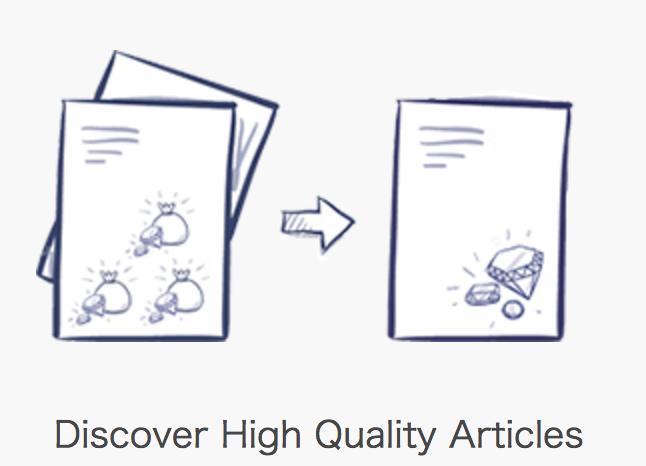
\includegraphics[scale=0.4]{img/discoverarticle.png}
\end{center}

2. プラットフォーム価値がユーザに還元される

\begin{center}
	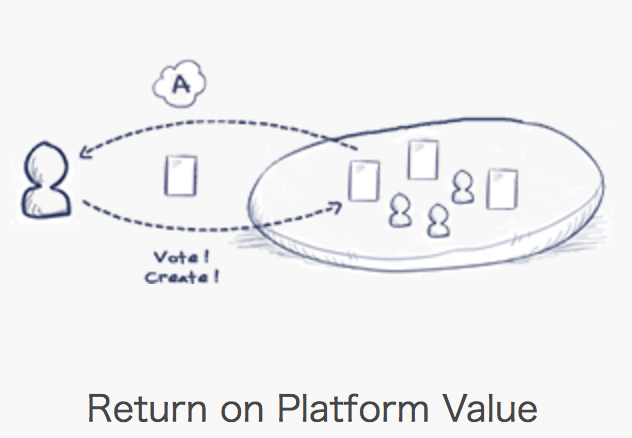
\includegraphics[scale=0.4]{img/returnvalue.png}
\end{center}

3. ブロックチェーンによりデータの高信頼性を従来よりも低コストで実現できる

\begin{center}
	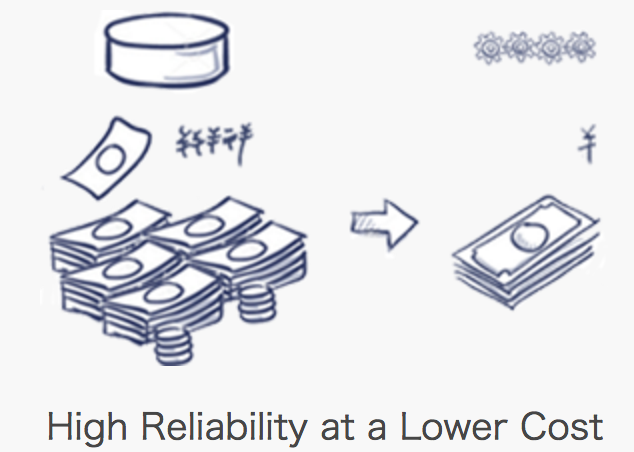
\includegraphics[scale=0.4]{img/highreliablility.png}
\end{center}

詳細の説明はLP(https://alismedia.jp)にも記載してあるためご参考いただきたい。

\section{我々が狙うマーケット規模と日本マーケットの魅力}
我々が長期的に狙うマーケットについては2017年の予測でSNS:5.6兆円、Webメディア:17兆円、合計:22.6兆円の市場である。なおかつ
これらの市場は2014年から急激に成長しており(全体で47\%の成長、SNSだけに絞ると130\%成長)、非常に有望なマーケットである。

\begin{center}
	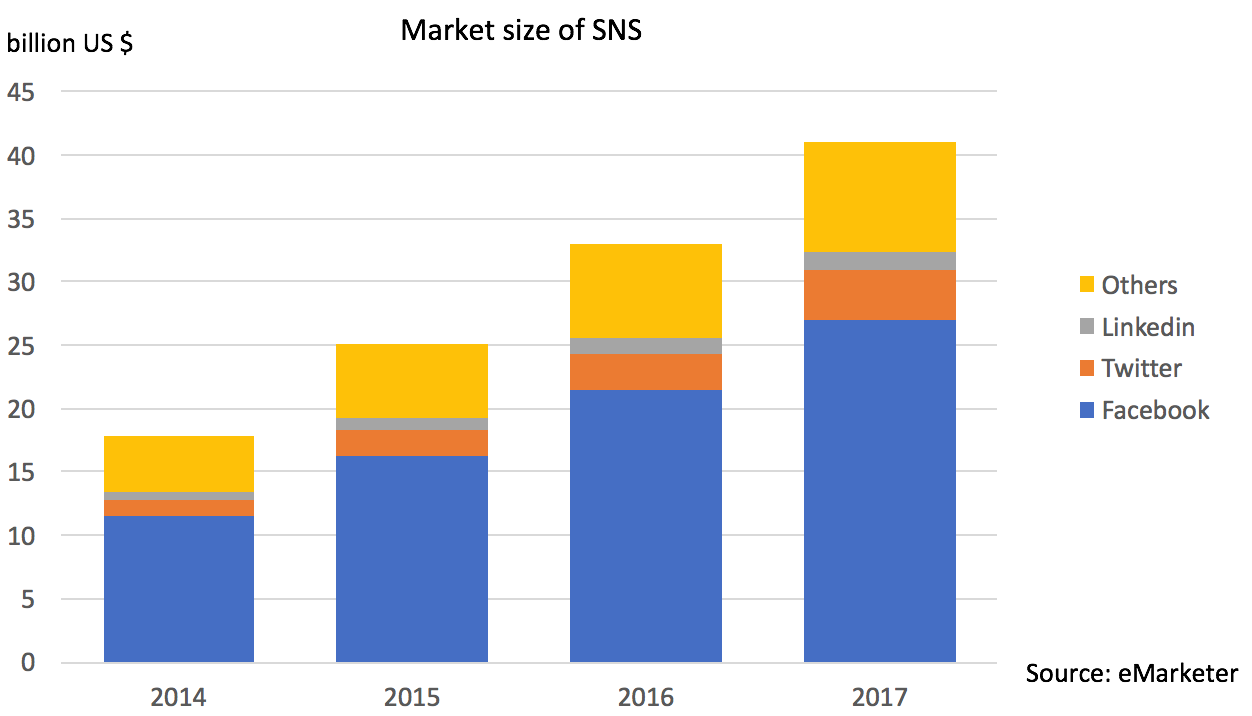
\includegraphics[scale=0.4]{img/sns-marketsize.png}
\end{center}

\begin{center}
	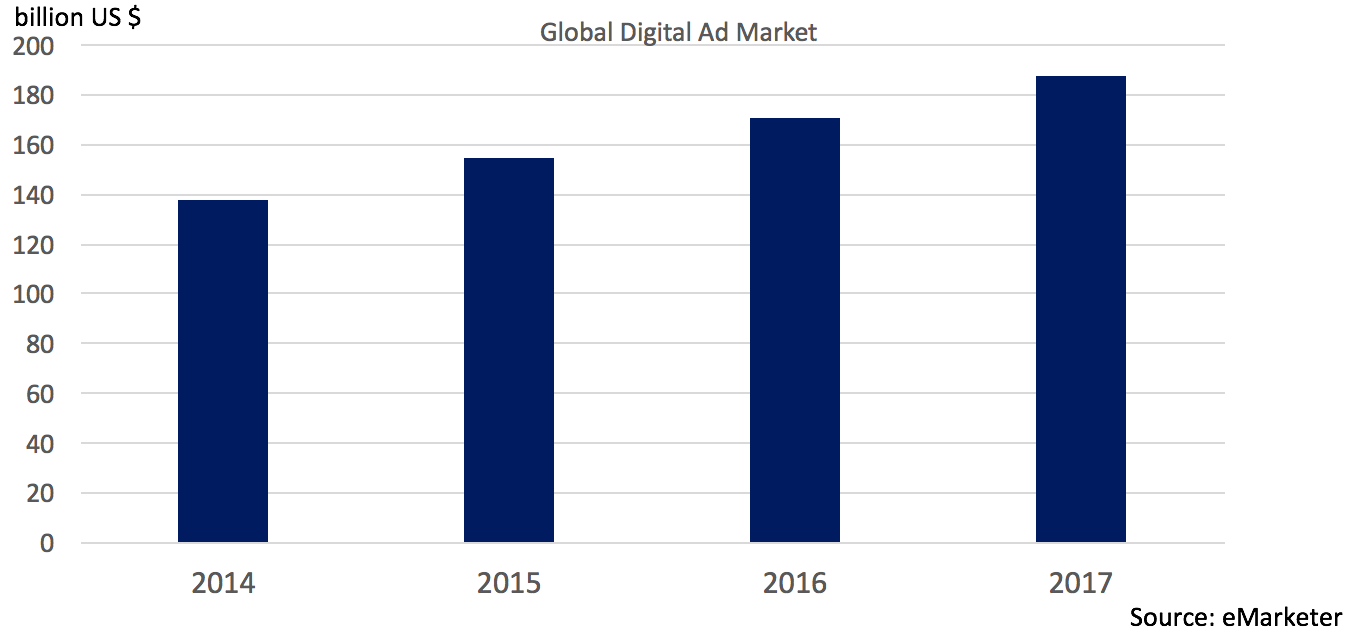
\includegraphics[scale=0.4]{img/digitalad-marketsize.png}
\end{center}

その中でも、一歩目としては日本のマーケットから攻めたいと考えている。まず、ブロックチェーン技術に関しては欧米諸国が先陣を切っており、
日本ではメインプレイヤーがほとんど存在しない。加えて、日本の改正資金決済法により海外プレイヤーは国内事業を運営できず、
国内プレイヤーについても事業者登録という大きなハードルを超える必要がある。
これは一度日本において先行者としてのポジションを確立すれば、言語という壁が逆に強固なものになり
独占的プレイヤーとしての立ち位置を確立することできる可能性を示唆している。言語の壁についてもMicrosoft社が同時通訳ツールを
すでにリリースしているなど、あと5年もすればほとんど言語の壁を意識することがなくサービスを利用できる世界が来ると予想している。
加えて、日本の名目GDPは49390億ドルと世界第3位であり、対外純資産は世界一を誇るなど未だに大きなマーケットであるといえる。
なおかつ日本のSNSとWebメディアの市場規模は最低でも1.1兆円はあると試算されている。
一方で、常に「日本語」という言語の壁を抱えていることが原因で、グローバルプラットフォームから
乗り遅れることが甚だしい(例えばWhatsApp, Tumblr, Pinterestなど、日本では存在すらほとんど知られていない)。しかしながら、
だからこそ日本は狙うべきマーケットであると我々は捉えた。
繰り返すことになるが、日本という世界的からみれば取り残されたマーケットで圧倒的なシェアを獲得し、その後グローバルマーケットに
進出するという方法は合理的な競争戦略に則った方法であり、我々のサービスの成功確率を高めるものであると考えている。
加えて主要メンバーが日本で生まれ育ち、言うまでもなくその文化とビジネスルールに精通しているため、
日本でビジネスをスタートすることは我々の現時点での最善策と言える。
\section{日本におけるプラットフォームのグロース戦略}
我々は日本マーケットにおけるサービスのグロース戦略として、3つのSTEPを想定している。

1. ニッチな領域のマーケットシェア確立(仮想通貨、マイナーなアニメ・漫画など)

2. あらゆる口コミサイトの領域に拡大する(飲食、旅行、ダイエットなどの日常情報から進学、結婚、住宅購入などのライフイベントまで)

3.蓄積された人の信頼情報をもとに、新たなサービスを展開する

まずは1.に関する説明を行う。ALISのFounderである
Masahiro Yasuはかつて日本におけるビジネスSNS(日本版のLinkedin)を開発していた経験がある。その経験から考える、
ソーシャルプラットフォームをグロースさせるのに最も大事な要素の一つは「ユーザからのフィードバック」である。この重要性はFacebookや
InstagramなどのSNSを使っているユーザであればわかると思うが、いかに多くのユーザが自分の投稿に対するフィードバックを
気にしているかという点でも明らかである。また、AARRRの文脈の中で
初期フェーズとして最も重要なものはChurn Rateをいかに下げるかであり、その重要な課題の一つが「ユーザからのフィードバック」なのである。
幸運なことに、この課題はトークン配布ロジックを実現することで解決することができると考えている。詳細のロジックは後述するが、
人々は「まだ誰も評価してないが、将来評価しうる記事を真っ先に見つけ出し、自分がいちばん最初にいいねをすること」という
行動原理にのっとって動くことが想定されるからである。これは報酬が
伴うALISならではのユニークな解決方法であり、経済ルールに埋め込まれているという強力なものであることに留意いただきたい。
また、グロースのための要因として重要だと考える2点目の要素は、Facebookやかつて日本でかつて成長したmixiなどのSNSに共通な
条件としてある「いかに内輪から始めるか」ということである。Facebookはハーバード大学のコミュニティーツールとして、
mixiは日本の大学のツールとしてどれも「内輪感」からスタートしている。
この重要性を戦術に紐付けるために、まずは「仮想通貨・トークンに興味がある人々」をターゲットとして記事を増やしていくという戦略を
取りたい。理由は明快である。

1.仮想通貨に関する情報はどれも信頼性の低いものが溢れており、人々は信頼のおける情報ソースを求めている

2.仮想通貨に関する情報はどれもクオリティの低い情報ばかりであり、役に立たない(ご都合主義のテクニカル分析を見せつけられ、○○は
上がるぞ!というtwitterを見て購入し、涙したユーザは何人いるだろうか。安心してほしい、私もその一員である)

3.何より我々ALISメンバーが仮想通貨・トークンが大好きであり、最も情熱を持って打ち込める記事である

からである。

上述を踏まえたグロース戦略の1.の概要をまとめると以下2点になる。

A. ニッチな領域×高信頼度を必要とするユーザが多い分野(初期は仮想通貨を想定)において、ユーザ集客を効率的に実施する

B. ユーザが参加後から多くのフィードバックを受けることができる仕組みを報酬を中心に準備する(タグ指定による新規記事の通知アラート、自分の投稿に対するコメントの通知アラート、など)

初期はあくまでも記事量が重要なため、良質な記事の投稿者に多くのトークンが配布されるロジックを組み込む。
しかしながらプラットフォームがグロースするにつれてこの割合は変更されるべきものであると我々は感じている。グロースの
タイミングに適切なキードライバーが最大となるように報酬の割合に関するパラメータ調整を実施したいが、それを我々が行ってしまうと
中央集権的になってしまう。よって、時期が来たらALISトークンを保有するユーザによる投票でどのようにパラメータを調整するかを決定したいと考えている。
参考までに我々が考えるサービス初期段階でのシステム図を貼り付けておく。この図はあくまでも現段階での仮設であり、実態に即して
何度でも修正されるべきものであることを注釈しておきたい。

\begin{center}
	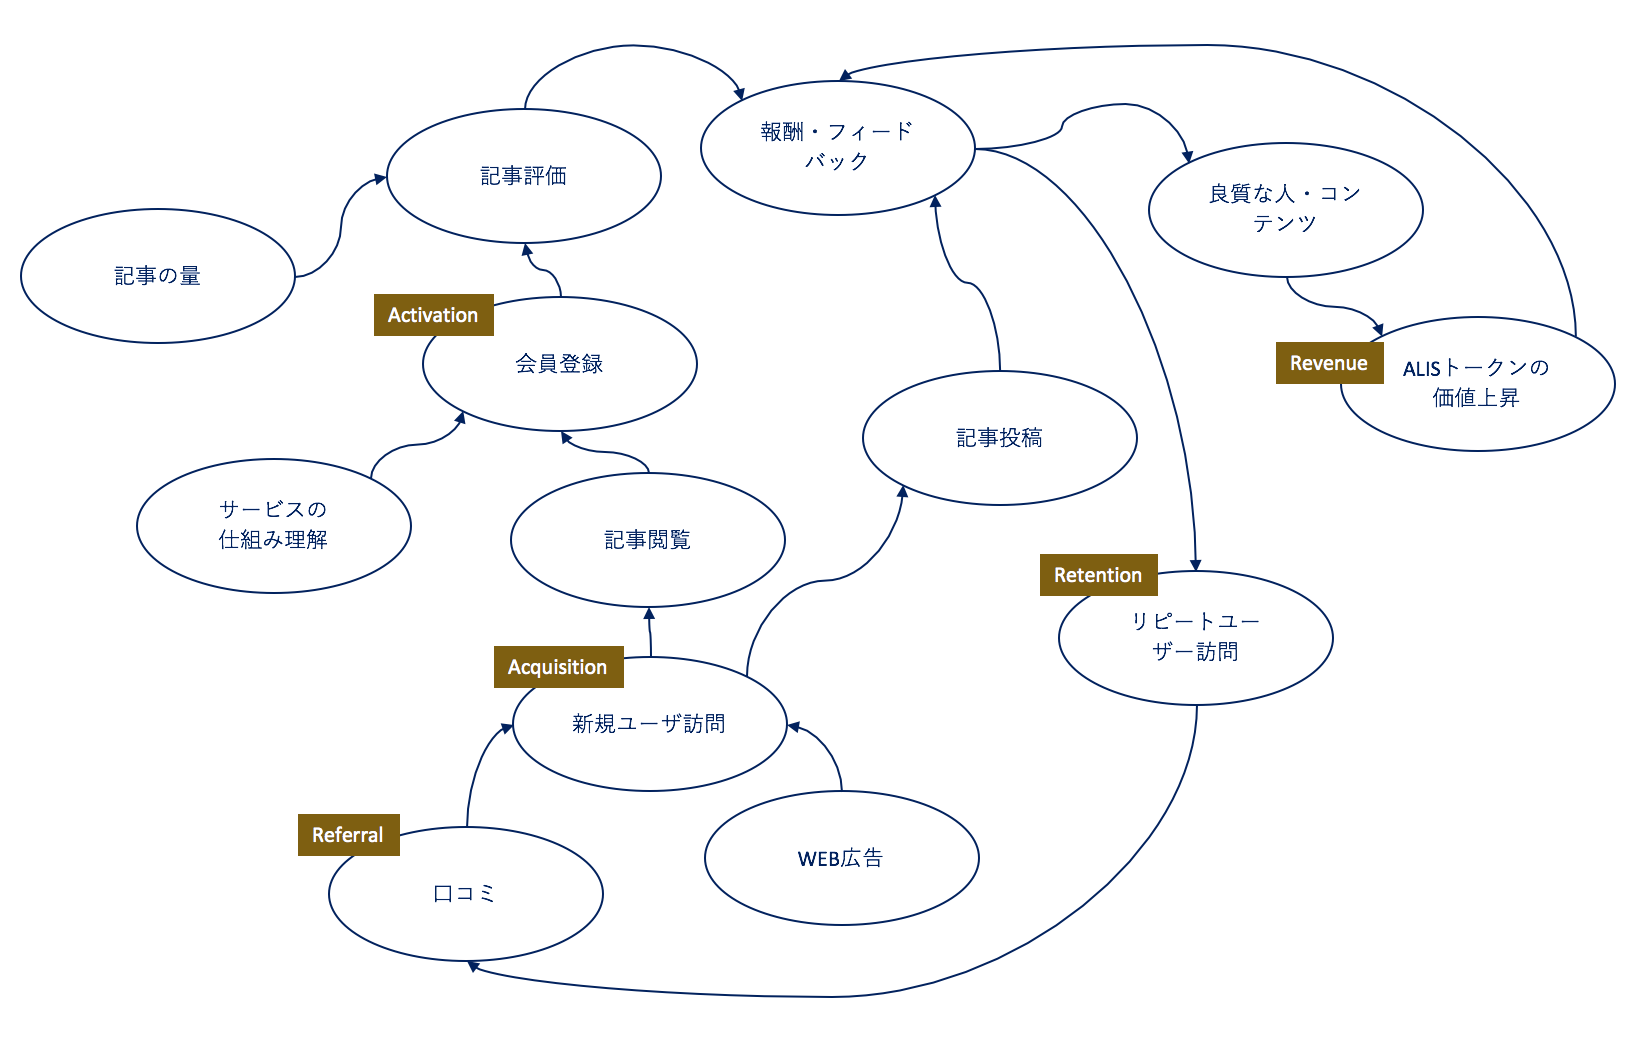
\includegraphics[scale=0.6]{img/systemthinking-with-AARRR.png}
\end{center}

上述した戦略がうまくいくと、ALISは「信頼できる情報・人が集まるプラットフォーム」としてのポジションを確立することが可能になる。
そのポジションを確立してから実施するのは

2. あらゆる口コミサイトの領域に拡大する

戦略である。これは飲食領域、旅行、ダイエットなどの
日常領域もしくは進学・結婚・住宅購入などのライフタイムイベントの領域で相性が良いと考える。なぜならば、人々はこれらの領域に
おいて、人の評判を元に情報収集することが多いからである。例えば日本におけるサービスだとyelpの日本語版である食べログやRettyが成長している。
このような領域が次のALISのターゲットであり、記事作成者・投票者ともに報酬を得ることができるというALISのUVPでディスラプトを狙っていきたい。

最後にもっとも長期的な

3.蓄積された人の信頼情報をもとに、新たなサービスを展開する 

について話をしたい。結論から言うと、我々は日本において仕事を受発注できるシステムをALISに構築することを考えている。
日本の国策として一億総活躍社会に基づいた働き方改革が推進されている(http://www.kantei.go.jp/jp/singi/hatarakikata/)。
詳細は割愛するが、重要な施策の一つとして人々の副業を推進するというものがある。なぜこの施策が重要視されるかを説明すると、
日本という国家は世界で類を見ない高齢化社会になっており、圧倒的な労働人口不足にとらわれている。そのような中で、
労働者ひとりひとりの生産性が最大化されているかというとそういうことはなく、もっと仕事を細分化し企業の垣根を超えて
個人が仕事をすることで生産性を向上させるという方法が模索されている。この推進を阻む大きな壁として
「個人の信頼度がまったく可視化されていない」ということが挙げられる。ここに対して、我々はALISを通じて蓄積してきた信頼データを
活用することができると考えている。これは我々の仮説ではあるが、良い仕事をする人は良い情報発信を行っていることが多い。
もっと直接的に言うと、良い仕事をする人は人から信頼されていることが多い。つまり、情報発信および情報発掘を行いながら
溜まっていた信頼データは仕事においても活用できるものであると考えており、国策に紐付けたエコシステムが実現可能であると考えている。
このエコシステムを実現した場合、報酬のやりとりが当然発生することになるため、
ALISトークンの通貨自体としての利用価値も高めるためにwalletとしての機能も強化することを想定している。
具体的にはALISの法定通貨との交換所の設置、他の仮想通貨との交換機能の実装などを予定している。

次章以降では、ALISの具体的なプラットフォームに関する説明を行う。
\section{プラットフォームの紹介と特徴}
ALISは、人々が良いと思う記事を作成したクリエイターおよびそのような記事を評価をした人々に対して、より多くの
ALISトークンを配布する。つまり、報酬により信頼できる記事・人を発掘することができるソーシャルメディアプラットフォームである。
そもそもこのようなメディア自体がかなり新しい概念のものになるため、すでに存在する類似サービスのSTEEMと
比較をした際の我々のプラットフォームの特徴を説明すると、

1. 我々のトークンは一つでシンプルであることにより、プラットフォーム発展のルールもシンプルであること

2. あえて仮想通貨の不安定性を許容し、インフレ率をSTEEMよりも抑えることで長期的なプラットフォーム維持を実現していること

3. 最終的なゴールを「人の信頼を可視化する」ことにおき、国策と紐付けて推進するというビジョンを持っている

という3点である。それぞれの特徴については次章以降におって説明をしていく。
\section{なぜ良質な記事が集まるのか}
人々が良いと思う記事を作り出す、もしくは評価するために必要なことは何であろうか。  
それはより多くの人が認める記事を作り出すあるいは発掘した人に多くの報酬を支払うということである。
また他者へ貢献できること、承認欲求が満たされること等の人間の根源的な欲求も大きな動機と言えるだろう。
それらの欲求が適切に満たされるよう設計することはソーシャルメディアプラットフォームを作る上での大前提である。
そしてALISの報酬システムは、その欲求と両輪を成してユーザーにより強い動機付けを行う。
記事作成者については、自分が作成した記事がより多くの人に、
かつよりALISトークンを多く持つ人に評価されることでより多くの報酬を得ることが可能になる。また、良質な記事の評価者に対しても、
誰よりも早く、かつ多くの人が良いと認める記事を評価することでより多くの報酬を得ることができる。これらに加えて、ALISトークンを
多く持っている人であるほど報酬の量は増えていく。つまり、よりALISトークンの報酬を得れば得るほどより良質な記事を生み出す
もしくはより良質な記事を発掘するインセンティブが働き、更に良質な記事が集まるというグッドスパイラルを形成することができる。
これが良質な記事が集まる理由である。このモデルをAARRRを元にしたシステム図(下図参照)に置き換えて説明しても同じことが言えることより、
やはり報酬がプラットフォームの成長を加速させるキードライバーであることがわかる。
以上、報酬の金銭面についてのみ記述したが、この報酬はまた前述の承認欲求とも不可分である。報酬は数値的に明示される性質上、ユーザーが
他者やプラットフォームへの貢献度合いを明確に実感できる指標となるからだ。金銭面を無視しても、純粋に承認欲求の文脈において
Facebookにおける「いいね! xx件」等と類似の効果が期待できるかもしれない。
	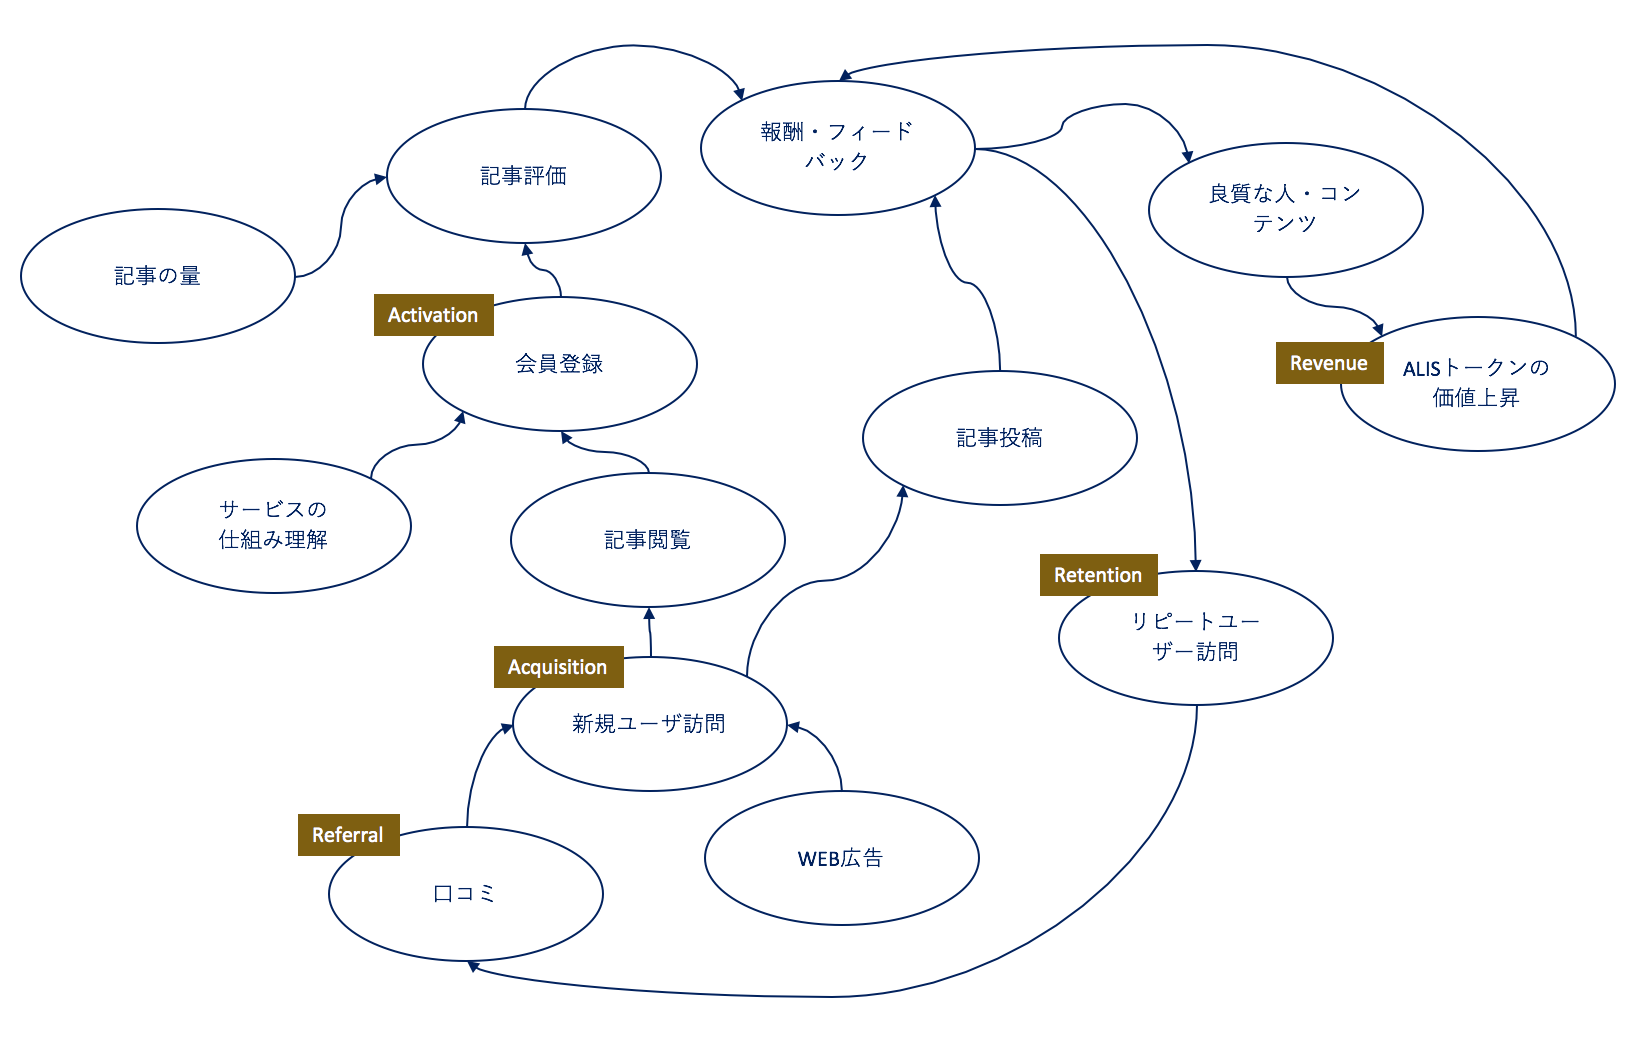
\includegraphics[scale=0.6]{img/systemthinking-with-AARRR.png}
\section{なぜ人々に価値を還元できるのか}
我々のトークンはそれ単体では価値を持ち得ない。しかしながら、ALISのプラットフォームの価値が
あると認められれば認められるほどALISトークンが価値を持ち、取引所で高値で取引されるようになる。一見懐疑的に思われるかも
しれないが、STEEMは同スキームですでに\$3.78億の評価を得ていることからこのスキームは実現可能であることが証明されている。
また、STEEMをフォークしてロシア語で作り変えたサービスのGOLOSも\$10億以上の評価を得ている(2017/07/17 現在)ことからも、
このスキームが成功する可能性が高いことを読み取ることができる。
\section{なぜALISは長期的な発展を続けることができるのか}
ALISが真に価値のあるプラットフォームとして認められるために最も重要なファクターがある。それは、ユーザーが粘着性を持ってずっと
使い続けたいと思うプラットフォームを提供することである。そのための方法はいくつかあるが、一つのこだわりとしてトークンの性質を
取り上げたい。我々のトークンは、プラットフォーム上で有効化されている(本章の後述の説明を参照)場合のインフレ率が50\%であり、この
インフレ分がALISトークンに貢献してくれたユーザへ配布されることになる。
これは、昨今の仮想通貨が取引目的ばかりにexchangeで扱われていることに関する危機感から設定された数字である。
ALISトークンを所有し、プラットフォームを発展させようと努力する人であればあるほどより多くのトークンを得ることができる仕組みづくりが
重要であると考え、50\%のインフレ率を設定することとした。しかしながら、
この条件だけであればトークンをALISに預けたあと、トークンが増え次第すぐに引き出してexchangeで売るというインセンティブを防ぐことが出来ない。
そこで我々ははNEMのPoI( http://nemmanual.net/NEM\_Technical\_reference\_JA/PoI/7\_PoI.html )から着想し、トークンを移してから実効性をもつまでには
時間が必要であるというロジックを導入する。
具体的な式は以下である。
\begin{align}
f(t) = log_{94}(t-1)\:(1 ≦ t < 94)
\end{align}
\begin{align}
f(t) = 1\:(t ≧ 94)
\end{align}
ここでtはトークンをALIS上のwalletにうつしてから経過した日数である。上記数式を採用した理由は3点ある。1点目は、新規ユーザが
早くALISの魅力を体感することができるよう、tが小さいときには上昇幅が大きいということ。2点目は、長くユーザが使うことで100\%ALISの
トークンの恩恵を受けることができるということ。3点目は、一度引き出してしまうとまたゼロから有効化させる必要があるため、
簡単に引き出しくないインセンティブをユーザに与えていることである。真にALISに貢献したいと思うユーザであればあるほど
この数式が合理性を持ち、長期的なプラットフォームの発展に貢献することができると考えている。
\section{トークンはどのように作成・配布するのか}
ALISはICOによって資金を調達する予定であるが、初期に5億枚を発行しその半分をEthereumとの交換を実施する予定である。
配布分の上限は2.5億枚であり、残りの2.5億枚については我々や我々のステークホルダーが所有することになる。我々が2.5億枚と
全体の50\%を保有する理由として、我々自身がプラットフォームを発展させるという健全なインセンティブを持つためである。
しかしながら、トークンの保有量を我々が最も保有しているからと言って、プラットフォームの価値を創造する決定権を我々が持つわけ
ではないことにご留意いただきたい。加えて我々はこの所有トークンを無闇矢鱈に売ることはない(後日公開する予定であるが、
我々はスマートコントラクトによりトークンを販売できない制約を設定する予定でいる)
さて、ICOによてt配布されたALISトークンについてはインフレ率が50\%のトークンであるとお伝えしたが、
そのインフレ分がどのように配布されるかを説明する。基本的な思想は先述のとおり2点であり、

1.素晴らしい記事を作ったと認められた人に配布される 

2.素晴らしいと人々が認める記事にいち早く評価した人に配布される

ということである。
この配布量について、ALISトークンの所有量が多ければ多いほど配布量を多く受け取れるというロジックを構築する。つまり、長くALISの
プラットフォームに貢献をし、トークンを多く保有する人たちを最も重要なステークホルダーと捉え、彼らがより恩恵を得られることを
ルールとして設定する。これはPoIの仕組みに近しいものであり、プラットフォームが壊れてしまうと困る重要度の高いユーザであれば、
プラットフォームへの健全な貢献を心がけるはずであるという前提に則っている。また、そうなると大量のALISトークンを買い占めたものが突然
プラットフォームに参入し、プラットフォームの価値を自分の都合の良いものに変えてしまうのではないかという懸念が生まれるかと思う。
この懸念に対しては、ALISトークンがプラットフォーム上で実際に有効になるまでには時間を要すると
いう対応策を先述のとおり講じている。つまり大量のトークン所有のユーザがすぐに不正を働くことを防止しつつも、トークンをプラットフォーム上
で保持し続けるというインセンティブも生むことができ一石二鳥の手法であるといえる。
\section{詳細の配布ロジックとパラメータの調整について}
まずALISの全体の発行量について言及しておこう。先述の通りALISは初期発行枚数として5億枚を予定しており、
そのうちの最大2.5億枚をcrowdsaleで販売する。売れ残ったALISに関しては我々チームが引き取るが、3年間は引き出せないよう
スマートコントラクトで縛る予定である。Crowdsaleを通じて配布したALISトークンのうち、
exchangeのwalletに入っている割合をx1,ALISwalletに入っている割合をx2とすると、x2に対して50\%のインフレ率が適用される。
このインフレ率分のトークンが、記事を作成する人と記事を評価する人に配布されることになる。この配布の詳細ロジックを
述べるわけだが、まずは我々の原則の考え方を共有しておきたい。

1. 記事の作成者と評価者はどちらも尊重されるべきだが、記事を作成するほうが労力がかかるため作成者への配布割合を重くするべきである 

2. 記事の作成者は自分が投稿した記事がいいねを集めれば集めるほどコインを配布される。同様に、記事の評価者は多くの人が良いねと予想する記事に投票するほどコインを配布される。 

3. コインの配布量やロジックは、プラットフォームの発展に伴い変更すべきである 

以上により、我々はインフレ分のALISトークンのうち、
90\%を作成者、10\%を評価者に配布するロジックを設定する(もし我々がICOの最低調達額3.5億円を達成した場合、
1年目については投票者には6700万、投票者には750万円が全体で配布されることになる。 *ただし、ALISの価値が全く変動しないと仮定した場合)。
これは、初期においては記事の量が集まることが重要であると考えているからである。しかしながら、記事の量が集まった次に重要な指標は記事の評価に徐々に変わって
いくだろう。その場合には評価者への配布量を増やすべきであると考える。これらのパラメータについてはプラットフォームの
段階に応じて調整されるべき値であると考えているが、その調整を我々運営者が実施するのは非常に中央集権的になってしまう。そこで、
我々はコミュニティよりこのパラメータの調整を要望された場合、ALISトークンの所有量に応じた投票を実施し、コミュニティの総意
(51\%以上の同意)を持ってパラメータを変更する運営方法を取ることを将来的には検討している。
次に、作成者・評価者一人ひとりに具体的にどのようにトークンが配布されるかを述べる。
まずベースとなるのは記事に設定されるベースポイント$A_{i}$である。このベースポイントは作成者・評価者それぞれの行動によって
算出される。ALISトークンを多く保有している投稿者が投稿した記事にはより多くのベースポイント$A_{i}$が設定される。具体的には、
\begin{align}
A_{i} = \frac{\rm Valid\:ALIS\:tokens\:owend\:by\:the\:user}{\rm ALL\:valid\:ALIS\:tokens}\:(A_{i} = 0.01\:{\rm if}\:A_{i} < 0.01)
\end{align}
が設定されることになる。 ALISを多く保有している人
ほどプラットフォームを健全に保つインセンティブが働くことと、連続投稿した記事に関しては不正の可能性が高いということを
鑑みてこのような設定になっている。投稿者についても同様に評価者ポイント$B_{i}$を持っており、
\begin{align}
B_{i} = \frac{\rm Valid\:ALIS\:tokens\:owend\:by\:the\:user}{\rm ALL\:valid\:ALIS\:tokens} * \alpha * (-\frac{1}{n}x_{i}+1) \:(B_{i} = 0.001 {\rm\:if\:} B_{i} < 0.001)
\end{align}
をパラメータとして持っている。ここでαは評価を行った当該ユーザが5分以内に別の記事を評価していた場合0、そうでない場合1になる
パラメータである。また$-\frac{1}{n}x_{i}+1$については、nが当該記事が報酬を承認されるまでに評価を行った総ユーザ数、$x_{i}$が当該ユーザが
そのうち何番目の評価をしたユーザかを示しており、早く評価を行ったユーザであればあるほど多くのポイントを保有するロジックになっている。
これらのユーザがいいね$B^{good}_{i}$もしくは低評価$B^{bad}_{i}$をすることになるが、ある記事に対するすべての評価ポイント$B^{good}$は
\begin{align}
B^{good} = Σ (B_{i} * θ)  * δ 
\end{align}
となる。ここで、θはユーザが自分自身の記事を評価した場合は0、そうでない場合は1になるパラメータであり、
δは記事に評価したユーザ数が10未満の場合は0、10以上の場合は1になるパラメータである。また、同じように
ある記事に対するすべての低評価ポイント$B^{bad}$は
\begin{align}
B^{bad} = Σ (B_{i}) * δ
\end{align}
として計算される。最後に、当該記事の総ポイントZを計算する式は以下となる
\begin{align}
Z_{i} = A_{i} + B^{good} - B^{bad}\:( Z_{i} = 0 \rm \:if\: B^{bad} > 2*B^{good})
\end{align}
この$Z_{i}$が記事の作成者のポイントとして設定される。また、
いいねをした個人がもらえるポイント$B^{good}_{i}$に関しては$(Z - B^{bad}) / Z * B^{good}_{i}$が自分のその記事に対するいいねポイントになる。
低評価をしたユーザは基本的にポイントはもらえない仕組みになっており、あくまでも不正防止観点で導入していると理解していただきたい。
あとの計算は簡単である。投稿者は自分の記事ポイント/総記事ポイント * インフレ分ALIS * 0.9を受け取り、投票者は自分の
投稿ポイント/総投稿ポイント * インフレ分ALIS * 0.1を受け取ることになる。なお、本項のロジックはこれが確定版というわけではなく、
サービスのグロース状況に応じて適宜変えるべきものであることを留意しておきたい。この変更に関しては我々が独断的に行うのではなく、
ユーザの投票を持って行うことを想定している。
上記説明のみでは具体的なサービスの画面イメージや機能がイメージしにくいかと思うが、現在設計・開発中なので出来しだい皆様に共有する。
\section{不正はどうやって防ぐのか}
上述の配布ロジックに従うと、トークン取得に関して次のような不正をユーザに許し、大多数のユーザが不利益を被ってしまう可能性がある。

1.ユーザが複数のダミーアカウントを作成し、自身が作成した記事に積極的に投票を行うことによるALISトークンの取得

2.特定のユーザが結託をし、指定した記事に対して積極的に投票をしトークンを取得する

我々はこれらの不正を防ぐための策をすでに
用意してある。まず一点目に関しては容易にダミーアカウントを作成出来ないような対策を行う。具体的にはSMSによる本人確認認証もしくは、
facebookアカウント連携による登録導線のいずれかにて対応を行う。また、二点目に関しては、

1. 特定ユーザがある記事に投稿し、時間をあけずに別の記事に投稿した場合はその記事の投票に対する評価は無効とする(なぜなら、そんなに短期間でいくつもの記事を読みうるユーザのほうが統計学的には少ないはずだからである)

2. Bad評価をされた記事のBad評価の割合を見て不正を働いていると思しきユーザへの配布を無効にする

などの対応により不正に対処していく。これはSTEEMがすでに採用している
不正防止ロジックから着想を得たものであり、STEEM自体がうまく動いていることから我々のプラットフォームでもうまく動作することが期待される。
\section{ALISで用いるブロックチェーン技術について}
言うまでもなく、我々の目指す人々の信頼性の担保という用途に最も適した技術こそALISの基幹技術であるブロックチェーンだ。
最高水準の信頼性が必要とされる通貨・決済を、中央管理者不在で世界規模で実現させたビットコインに代表されるように、こと信頼性の担保という文脈において
ブロックチェーンは既存技術に比べて圧倒的な優位性を誇る。これは、まったく比較にならないレベルで、根本的に格が違う。
ビットコインが実現したパラダイムなどはもはやアートの領域であり、我々はこの前人未到の社会変革に
畏敬の念を覚える者である。これがALISを立ち上げる原動力となった。
現状、少なくとも日本においてブロックチェーン上に人々の信用情報を構築した前例は無い。
そして一度これを構築できた場合、容易に覆しようのない圧倒的な優位性を担保できると確信している。
ピーター・ティールの言うところの成功企業の必須条件である「独占」を、これ以上無い形で実現できるためだ。
我々はブロックチェーン技術をユーザが作成した記事の評価および報酬データの保存に用いる。この保存作業を
承認するのはALISコインをwalletに入れvalidされたトークンを持つユーザである。これらのユーザは
計算された先述のトークン配布のためのポイントが適正かどうかを判断し、各ユーザに適切に配布することになる。
最も不正が起きやすいコインの配布という部分にブロックチェーン技術は相性が良いため、このような技術選定を行っている。
また、我々は現在EthereumやMicrosoft Azure(我々は現在Azure BizSparkパートナーとして
Microsoft社から認定されており、BizSpark+としての審査も受けることになっている。)などの技術のうち、どの技術が最も高信頼・低コストを
実現できるかを検討中である。本章についてはまだ技術的な検討が完了していないため、追加の情報が出次第追記していくことを約束する。
現時点では少なくとも評価・報酬の部分はブロックチェーン技術を活用することを想定しているが、その他の機能については
別の技術も検討した上で慎重に決定したいため、現在選択肢を模索中であるということをご認識いただきたい。
\section{チームのビジョン・ミッションおよびチームメンバーの詳細プロフィール}
我々ALISのチームのビジョン・ミッションは明確である。ビジョンは、世の中の有益な情報と人を可視化することにより、CtoCでの経済圏の
成長スピードを加速させることである。日本という国家においては、人口減少が国家問題として重くのしかかっている。この重しを
取っ払うためには国民一人ひとりの生産性を向上させることが必須であり、国としても一億総活躍社会というビジョンを掲げ、働き方改革
というミッションを遂行している段階にある。国民一人ひとりの生産性を向上させるには様々な方法があるが、もっとも重要なことの一つは
「一人の人間が関わる仕事の幅を増やすこと」である。いわゆる副業と呼ばれるこの方法は現在日本において積極的に推進しようという動きが
加速しているが大きな問題がある。それは、一個人が仕事をすることになる以上、一個人の信頼性を担保しないことには結局は絵に書いた餅で
終わってしまうことである。我々はこの問題に対して、信頼できる記事と人との出会いというネットワーキングを通じ、解決するような
方法がないかを考えていた。つまり我々のミッションは、

1.報酬によって有益な情報・人と無益な情報・人とを区別することができる

2.どんなに信用がない個人でも、有益な記事を創造あるいは発掘した個人に信用を付与すること

3.それを人々が自律的な経済圏で営めるプラットフォームを実現すること

である。ビジョンに対して真っ直ぐな思いをもった我々であるからこそ成し遂げられると自負しているし、
我々がやるべきだという使命感を抱いている。また若干手前味噌感が拭えないことを承知しながら記載するが、
コアメンバー全員が経営・ビジネス戦略・サービス開発・マーケティング・エンジニアリングに
ある程度精通しつつも、自分の得意分野を持っているというバランスの取れたチームになっている。
以下に我々のチームの主要メンバーのプロフィールを掲載しておく。
もちろんこの他にも大勢の協力者がいるが、我々は名前だけを借りるような無意味なプロフィールメンバーを
増やすことは支援者に対して誠実ではないと考え、コアメンバーのプロフィールのみを掲載している。
もし我々に興味を持っていただいたのであれば、ぜひslack(https://alis-slack.herokuapp.com/)にご参加いただきたい。
我々はなるべく皆様とコミュニケーションを取ることを心がけているため、どのような質問でも可能な限りお答えする。
\begin{quote}
	
\includegraphics{img/yasu.jpg}
	
Masahiro Yasu

Founder

Yasu is a graduate from Kyoto University, the university with the highest
number of Nobel Prize winner recipients in Japan. He majored in nuclear fusion and 
analyzed alfven eigenmode raised in helical plasma by Fortran. After graduation, 
he joined Recruit Co., Ltd. (The 2nd largest HR company in the world, also 
the parent company of Indeed). Yasu is experienced in business development, 
including business strategy and system development of several products, 
such as business SNS and referral tool. He also actively worked on machine 
learning and natural language analysis, and received the GROWTH FORUM 
Award which is the highest prize in Recruit. Currently he also serves as a 
project leader of a joint project with Microsoft Japan.
\end{quote}
\begin{quote}
	
\includegraphics{img/mizusawa.jpg}

Takashi Mizusawa

Co-Founder / Marketing

Takashi started a venture company as a university student. After graduation 
he started his career at the worldwide famous Benesse Corporation. After winning 
the company's annual MVP in his first year, he worked mainly in business 
development such as student SNS and education services on tablets. After working 
at Benesse for 6 years, he joined Recruit Career Co., Ltd., known for connecting 
"learning" and "working". There he gained experience in business development of 
MOOC and referral tool. He is interested in using social networks in HR. 
He envisions a world where individuals can earn success through their own unique abilities.
\end{quote}
\begin{quote}

	
\includegraphics{img/ishii.jpg}

Sota Ishii

Co-Founder / Engineering

Sota has over 13 years of experience as a system engineer. He took on the 
role as a development leader of a famous Japanese HR company. During his 
time there, he created an award-winning HR system that contributed to the company's 
service growth. He is interested in new technologies and business, taking on roles in 
varies positions. He strongly believes that blockchain technology will be a widespread 
standard within in a few years. Due to the recent rise of crypto currency, he has 
committed himself to the ALIS project.
\end{quote}
\begin{quote}

	
\includegraphics[scale=0.3]{img/erichin.jpg}

Bato Erichin

Communication / Engineering

Erichin is a graduate from Tsinghua University, majored in Thermal Engineering. 
He received master's degree in the Chinese Academy of Science, focus on 
supercomputing base large-scale parallel CFD. After graduation in 2014, he 
joined Recruit Co., Ltd., and now is a full stack engineer. He has skills such as 
iOS, Android, frontend, backend and UI/UX design. He also has a role as a bridge 
of communication for our Chinese user on Weibo, Wechat, and other famous SNS in China.
\end{quote}
\begin{quote}

	
\includegraphics[scale=0.3]{img/kamei.jpg}

Tatsuhiko Kamei

Regal department

Kamei graduated University of Tokyo, the most authentic university in Japan, 
After joining Recruit Career Co., Ltd. as a legal staff, he handles fields such as 
IT and web services, marketing, human resource and etc. He has special advantage 
in legal affairs of new business development. He also enjoys athletics in leisure time, 
especially triathlon and marathon.
\end{quote}
\section{ファイナンス}
トークンが将来どれぐらいの価値になるのかを楽観・中庸・悲観の3パターンで記載する。算出にあたってSTEEMの現在の評価を大いに
参考にさせていただいた。基本的なロジックとしては、STEEMにおける1ユーザの価値を参考に、我々のユーザ数の伸びにその価値をかけると
いう方法で算出した。ここで暗黙の前提としておいている以下の点にご注意いただきたい。

1. 1ユーザが平均2投稿をする(STEEMのユーザ平均値)

2. ユーザ数以外のあらゆる部分(運営メンバー、アプリケーションの素晴らしさ、利用ユーザの国など)はSTEEMと同等である

ここで算出した3年後の価値を、3年後に発行されているALISトークンの総量で割ったものが1ALISトークンあたりの価値になる。
具体的なシミュレーション結果は以下の表をご参照いただきたい。
	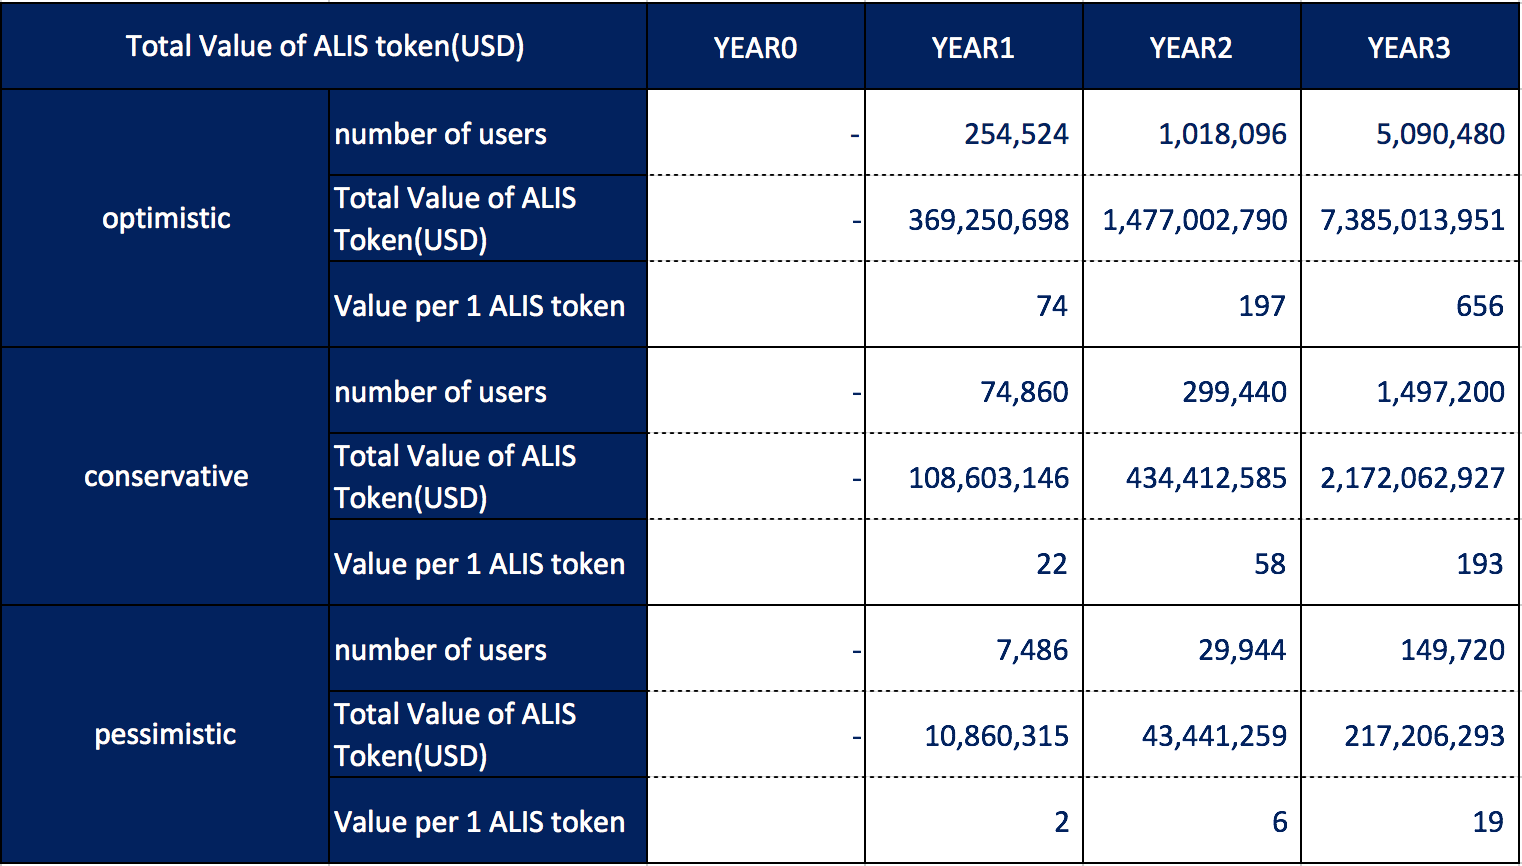
\includegraphics[scale=0.6]{img/financialtable.png}
算出のために用いた数字はすべて下記に掲載したのでご参考いただきたい。

\begin{center}
	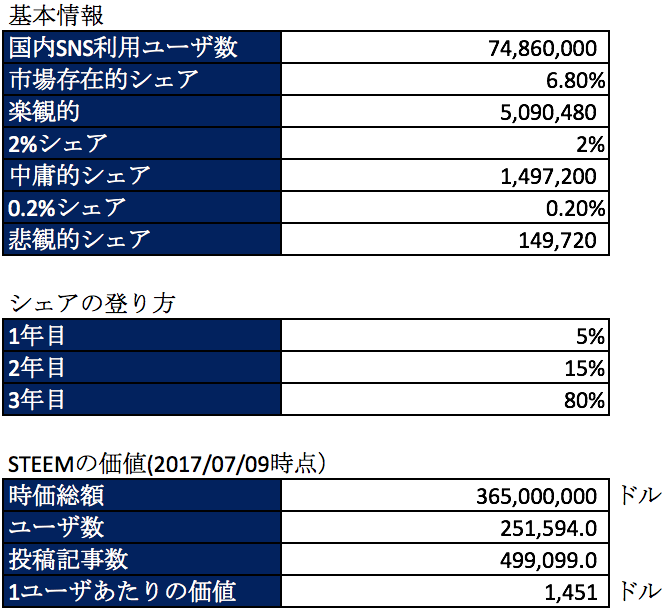
\includegraphics[scale=0.6]{img/base-info-of-finace.png}
\end{center}

これらの数字はあくまでも仮想通貨市場が長期的に伸びるという仮定をおいた場合の試算結果であることにご注意いただきたい。
\section{お金の使い道}
我々はクラウドセールの最低目標額3.5億を集めた場合、トークンを以下のような用途・割合で使う想定でいる。

1. 25\%: 優秀な開発メンバーのアサイン(特に優秀なUI/UXデザイナー1名、WEBデザイナー1名、フルスタックエンジニア4名。)

2. 25\%: ユーザ集客のためのマーケティング費用

3. 25\%: 国内事業者として認可されるための申請費用

4. 25\%: 初期に協力してくれたメンバーや今後協力してくれるパートナーに対する費用

3.5億円の調達をオーバーした分に関しては、基本的にはマーケティング費用にほとんどを投じる想定であるが、以下のような用途にも使用する可能性がある。

・より強いバックオフィス(経理・法務)の構築 

・ユーザサポートの強化(仮想通貨のサービスへの問い合わせは膨大であるため)

・固定のオフィスの準備(しかしながら我々はなるべく固定費を持たないために、資金に余裕が出るまでは固定のオフィスはレンタルしない想定でいる。少しでもプロジェクトの成功確率を高めるためである)

	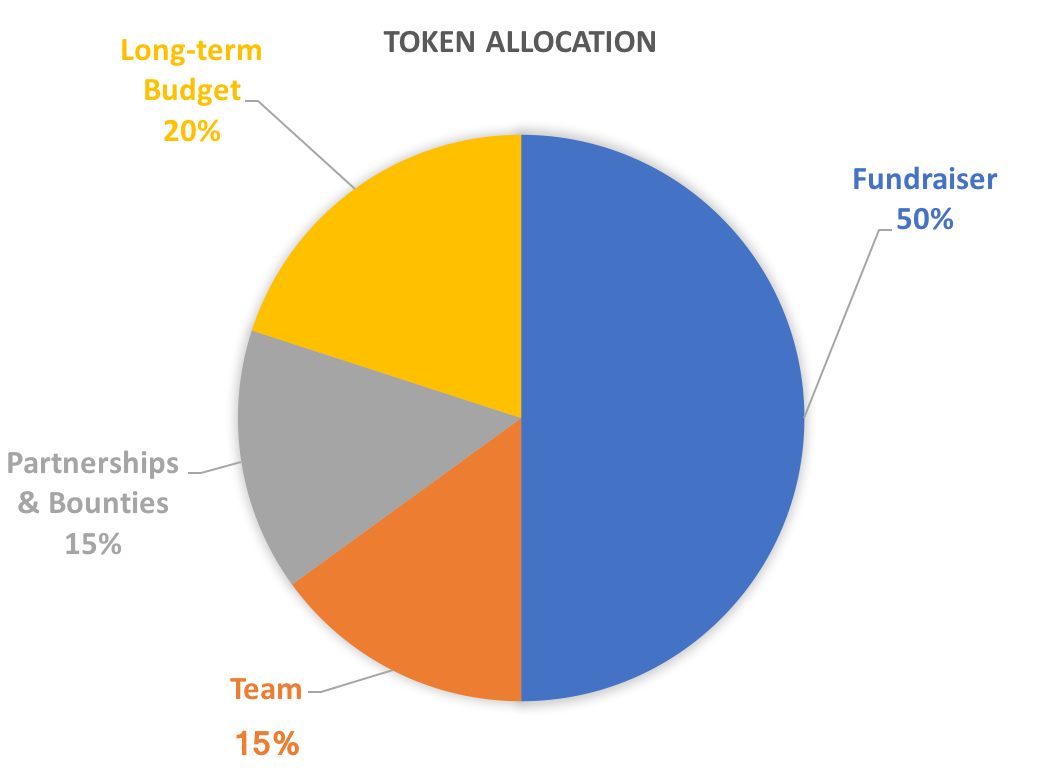
\includegraphics[scale=0.4]{img/tokenallocation.png}
	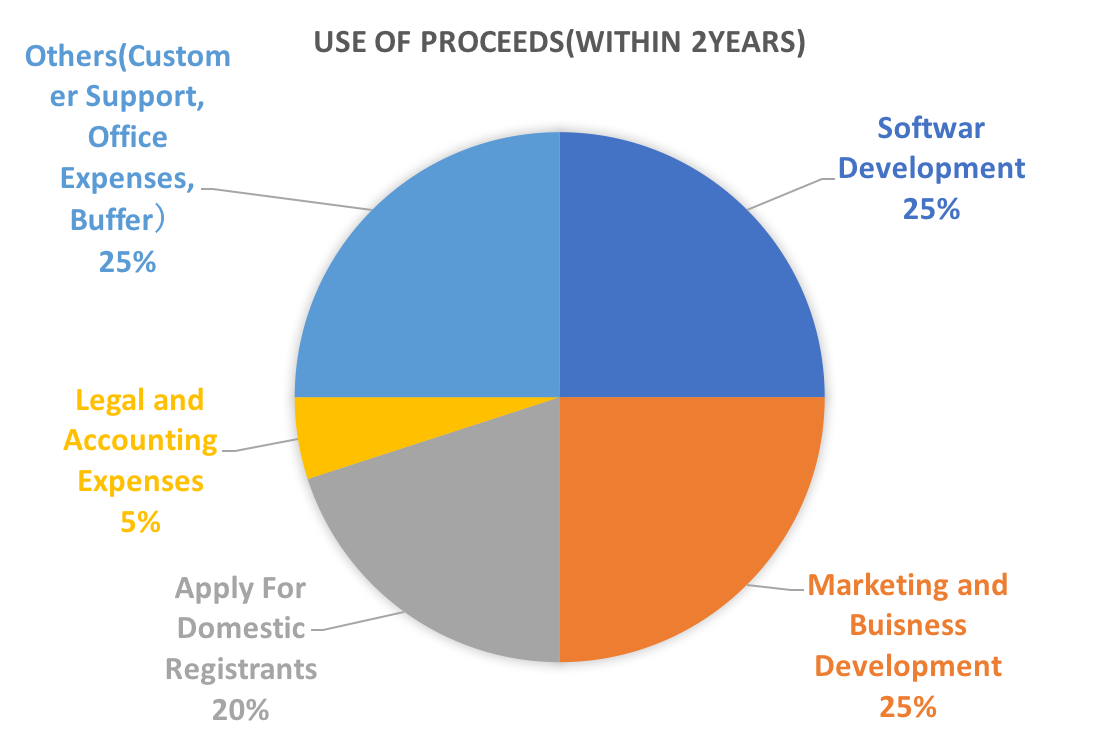
\includegraphics[scale=0.4]{img/useofproceeds.png}
\section{企業の運営方針}
我々は現在の株式会社はとても旧世代なものであると感じる。まずチグハグな点がすごく多い。会社は株主のものと言いながらも、
株主が知ることができる情報は株主総会での着飾られた情報のみである。またその経営権を託されている役員人は、自分が絶対正解だという
前提の元でしか決定をくたさず、現場社員にその決定を押し付けている。ゲイリー・ハメルが未来の経営でも書いているように、会社の
システムは数百年以上進化を止め化石化しており、我々はこの状況に1石を投じるべく以下のようなルールで経営をしていきたい。

1.プロジェクトの状況はtrelloなどを用いてすべて透明化する

2.メンバー間のコミュニケーションについてもできるだけ公開する

3.開発コードはすべてオープンソースとしてgithubに公開する

4.会社の方向性およびメディアのグランドルール変更については、トークンを所有する人の多数決にて承認とする

5.働く従業員の給与は従業員間ですべて公開する。 

加えて我々が調達する通貨は一人ひとりの個人の皆様から頂いたものである。その方々に対して、企業経営をできるだけ透明にすることが
義務であると考えているため、その文脈にのっとっても上記ルールは挑戦すべきものであると考えている。
正直どこまでこのルールを運用できるかは分からないが、
可能な限り次世代の経営に挑戦し、本当に会社を支えてくださる人々と一緒に運営できる組織づくりを目指したい。

\begin{center}
	
\includegraphics[scale=0.4]{img/thefutureofmanagement.jpg} \\
	ゲイリー・ハメル『未来の経営』
\end{center}
\section{なぜ香港でICOを実施するのか}
我々が日本でプラットフォームを開発するにもかかわらず、香港でICOを行うことに不安を覚える方が少なくないと察する。理由は明確で、
日本においては2017年4月以降国内事業者のICOが「改正資金決済法」(http://www.fsa.go.jp/common/about/20170403.pdf)の施行に伴い
禁止されたからである。我々も当初は日本でのICOを想定していたが、最近の国会での討論なども踏まえ、日本におけるICOは違法に当たる可能性が高いと判断し、
海外でICOを実施することを決断した。その中でも香港を選んだ理由については、最もコストを安く会社を設立・維持できる国であり、
なおかつ仮想通貨に関する規制がないことが大きな要因である。香港で調達したトークンを元に、日本国内における登録事業者申請を
行うことで国内ユーザも海外ユーザもなんの柵もなくトークンが取引できる状態を目指す。また、国内事業者になることで日本国内の
仮想通貨取引所に取り扱ってもらうことができるという大きなメリットが生まれる。我々は国内最大級の取引所とすでにコンタクトを取って
おり、将来の上場可能性と方法についても議論をしている。この事業者申請が完了するまでは、海外の取引所においてのみ取引可能な
トークンとなることをご留意いただきたい。また、香港の法人については当面ICO目的のためのみに存在する法人として扱うが、日本の
法律問題やその他の問題で日本法人での運営が難しい部分が出てきた際にバックアップする存在として長期的に維持していく想定でいる。
\section{結論}
長々と付き合ってくださったことに感謝をお伝えする。お読みいただいたとおり、我々は本気でこのプラットフォームの実現に燃えている。
我々の理想的な世界を実現するまたとないチャンスであり、なおかつそれを皆様のご支援をいただきながら挑戦できるチャンスであると
考えているからである。もし今まで述べた世界観の実現に賛同してくださるのであれば、ぜひともICOにご参加いただきプラットフォームの発展に
貢献いただきたい。我々は、皆様と新たなプラットフォームを構築できる日が来るのを楽しみに待つこととし、このホワイトペーパーを締めくくる。
\end{document}
